\chapter{Introduction}  \label{Chapter1}
\lhead{Chapter 1. \emph{Introduction}}

Supernovae (SN) are extremely luminous stellar explosions. At their brightest, they can outshine the galaxy that gave birth to them, making them visible at great distances and far back in time. SNe have been observed by stargazers since the dawn of humankind. By studying nebulae formed as remnants of past explosions, as well as ancient records we know that human history is filled with observations of `guest stars' most famously in 1054 where the SN, now observed as the Crab nebula, has been recorded in China, seen to be brighter than the full moon at night and visible during the day, as well as the SN1574, known as the Tycho SN and SN1604 in the end of the 16th and beginning of 17th centuries.

Despite their early observations, the term `Supernova' was not coined until 1934 when \citet{Baade1934} were able to estimate their absolute magnitudes. Using Cepheid variables, they measured the distance to several SN host galaxies and found them to be significantly greater than those of classical `novae'. The prefix `super' reflects their absolute luminosity which must be much greater than that of novae to explain their bright observed magnitudes.

\section{SN classification}
At that point of their discovery, little has been known about the properties and physical origin of these extreme objects, largely due to the scarcity of their observations at that time \citep{Zwicky1938}. In the years to come, many generations of astronomers built increasingly larger and more sensitive surveys, observing thousands of SNe to date \citep{Alsabti2017}. With this came our understanding of the various types and flavours of SNe and the breath of the variation in the objects that can give rise to such brilliant explosions.

\subsection{SN\,Ia}
Perhaps the most well understood and most heavily studies class are the thermonuclear SNe. While a number of their subclasses exists \citep[amongst others: SN\,.Ia, SN\'Iax, SN\,Ia-91T, SN\,Ia-91bg][]{Alsabti2017} all of these objects likely share a similar physical origin to the main SN\,Ia class. There are competing theories explaining their origin, both describe a thermonuclear explosion of a white dwarf (WD) star, but differing in the mechanism which triggers the ignition. In the single-degenerate scenario \citep{Whelan1973} a WD, in a binary system, accretes matter from a main-sequence or red giant star until it reaches the Chandrasekhar limit defined as the point at which the electron degeneracy pressure can no longer support the star against a gravitational collapse, resulting in an increase in pressure and subsequent thermonuclear ignition of its core. The alternative explanation suggests that instead of a single WD, a binary WD system interacts internally, spiralling down through the release of gravitational waves, resulting in their eventual collision triggering a powerful shockwave, sufficient to ignite the degenerate matter even at sub-Chandrasekhar limit masses \citep{Iben1984}. Both of the above mechanisms result in a production of $\sim$0.7M$_\odot)$ of Ni56 \citep{Scalzo2014} which decay radioactively to Co56 and Fe56 producing a vast quantity of high energy Gamma radiation, which is subsequently reproduced by the SN ejecta into visible light.

\subsection{SN\,II}
The origin of SN\,II in many ways mirrors that of SN\,Ia; both are the result of the end point of the evolution and the death of their progenitor star. SN\,II are born when a $>$8M$_\odot$ star exhausts all of its nuclear fuel at the end of the iron burning phase \citep{Clayton1983}. At that point, the core is supported purely by the electron degeneracy pressure and collapses shortly afterwards into neutron star under the gravitational pressure of the outer layers of the star. The infalling shells rebound of the, now, solid core and are further energised and accelerated by either the neutrinos released in the collapse of the degenerate core \citep{Burrows1987} or jets formed due to the accretion of the infalling matter onto the core \citep{Khokhlov1999,Burrows2007}.

In this process, only a small, in comparison to SN\,Ia, amount of the Ni56 is formed which alone could not explain neither the luminosity of these core-collapse SNe (CCSN) nor their light curve morphologies which are often associated with a sharp rise followed by either a long plateau phase (SN\,IIP) or a linear decline (SN\,IIL) \citep{Alsabti2017}. These are the effect of Hydrogen recombination (ionised to neutral) in the outer layer of the ejecta, resulting in a blackbody-like a spectrum with prominent P-cygni profiles visible in the spectra. Additionally, some objects also show narrow emission lines (SN\,IIn), of mostly hydrogen, which are the result of the interactions between the SN ejecta and extended material ejected by the progenitor star some time before the main event \citep{Pastorello2002,Sternberg2011}.

\subsection{SN\,Ib/c}
SN\,Ib/c have a very similar origin to SN\,II. They are also a result of a core collapse of a giant star but significantly they originate from larger and more `stripped' stars. These objects are often referred to as Stripped-Envelope SNe reflecting the fact that no hydrogen (SN\,Ib) nor helium (SN\,Ic) are visible in their spectra as they were removed from the surface of the star by either winds or coronal mass ejections a relatively long time period to the onset of the SN event. Some theories suggest that the stripping cannot be explained solely using wind and coronal ejections and must be a result of an interaction with a companion star \citep{Tauris2013}.

Thanks to the higher mass of the progenitor star, these objects often result in a larger production of Ni56, resulting in a higher luminosity and a morphology which in the extreme cases can closely resemble that of a SN\,Ia. Spectroscopically, this class of SNe shows a strong formation of Oxygen and Carbon and well as small quantities of other, intermediate-mass elements \citep{Filippenko1997}.

\subsection{Other subclasses}
Outside of the main, or most commonly detected, subclasses of SNe lives a number of rares and more exotic transient types. Amongst these, there is a number of intermediate classes of CCSNe that originate at the boundaries of the progenitor scenarios. This includes SNIIb, SNIbn and SNIbc amongst others \citep{Alsabti2017}, however, an overlap also exists between the SN\,Ia and the interacting CCSN. SN\,Ia-CSM are one of the most luminous classes of SNe as the extreme brightness of SN\,Ia is enhanced further by the interaction of the ejecta with a layer of circumstellar material (CSM) likely ejected by the companion star \citep{Dilday2012}.

As SN surveys become more sensitive and sophisticated, the numbers of known SN classes grew as well. In recent years, higher cadence SN searches have led to the discovery of a new class of Rapidly Evolving Transients (RAT) with an extreme variation in their peak luminosity ranging from -15 < M < -22 \citep{Pursiainen2018}. Little is yet known about their physical origins, however, their observations suggest a featureless blackbody-like spectrum, often associated with initially high temperatures followed by rapid cooling. A possible interpretation of these objects is an object which undergoes a direct collapse to a black hole, producing none or little Ni56, explaining the lack of a slowly declining light curve. In this scenario, the observed morphology is a result of the interaction between the SN shock with an extended shall of dense wind \citep{Piro2015}, similarly to an effect sometimes observed in superluminous supernovae (SLSN).

\section{Superluminous Supernovae}
Superluminous supernovae (SLSNe) are a recently identified class of transients defined as events with an absolute magnitude brighter than $-$21 ($M<-21$) \citep{Gal-Yam2012}. They appear 10-100 times brighter than normal supernova events, and form at least two distinct classes: SLSNe-II, which show signatures of interaction with CSM via hydrogen and other lines \citep{Ofek2006,Smith2006,Drake2011}, and SLSNe-I (or SLSNe-Ic), which are hydrogen-poor \citep{Quimby2011}. While SLSNe-II may naturally be explained as an extension of the fainter SN\,IIn events, the power source behind SLSNe-I remains a subject of debate \citep{Gal-Yam2012}.

SLSNe-I (SLSN; henceforth) are the protagonists of this thesis. In this section, I will introduce the observations that have led to their discovery, their spectroscopic and photometric properties as well as their host galaxies. Furthermore, I will introduce their most commonly accepted formation theories and their effect on the rate of SLSN.

\subsection{Discovery}
The observational properties of SLSNe had a strong impact on the timing of their discovery. As a rare but luminous class of transients, the probability of their detection was low in the early SN surveys in the local universe due to their lower sensitivity and search volume. The first signs of the existence of a new class of extremely luminous SNe came with the discovery of SN2005ap \citep{Quimby2007}, SN2006gy \citep{Ofek2007} and SCP06F6 \citep{Barbary2009}. In each case, the distance measurements for the objects have placed them at a luminosity $\sim$100 times brighter than ordinary SNe. However, the low quality of their early light curves and spectra along with a lack other example resulted in these objects being treated more as extremes of the known classes of objects instead of a separate new class.

This picture has evolved dramatically in the last decade with the onset of a number of deep, wide field surveys such as the Texas Supernova Search \citep[TSS;][]{Quimby2006}, the Palomar Transient Factory \citep[PTF;][]{Law2009, Rau2009}, the Supernova Legacy Survey \citep[SNLS;][]{Astier2005,Guy2010,Perrett2010}, the Panoramic Survey Telescope \& Rapid Response System \citep[Pan-STARRS;][]{Kaiser2010} and the Dark Energy Survey \citep[DES;][]{Flaugher2005}. With an increased sensitivity, longer observing season and a lack of host galaxy selection bias; each one of these surveys was responsible for detecting several SLSNe, jointly shaping our current understanding of this new and exciting area of SNe research.

\subsubsection{Luminous Supernoavae}
The terms `Luminous Supernovae' and `Superluminous Supernovae' became popular in the literature upon the discovery of SN2007bi \citep{Gal-Yam2009} during the science verification phase of PTF. Its light curve, containing only the single \textit{r}-band filter, lacked the rise time information but demonstrated a very slow decline consistent with the radioactive decay of a large mass of Ni56. At that time it was believed that such event could be a result of a Pair Instability SNe (PISN; \sref{sec:Origins}) and were therefore thought to be a new class of transients.

Following shortly from this, a number of objects were discovered with similar properties. \citet{Quimby2009} presented a sample of SNe detected by PTF along with the first, comprehensive sample of their spectra. While mostly consisting of a blue, featureless blackbody continuum, some absorption lines including CII, MgII and OII \citep[see ][for more recent line identification]{Mazzali2015} were identified in all spectra in this sample, confirming the redshifts and extreme luminosity of these events.

\subsection{Properties}
Beyond confirming their redshifts, the prominent UV spectral lines can also be used to measure the expansion velocity and temperature of the photospheres of SLSNe, measured around the maximum light to be of the order of $\sim$15000km/s and $\sim$10,000K respectively \citep{Inserra2013}. This suggests that SLSNe are a class of very energetic events powered by an internal engine capable to re-energise the ejecta to produce the observed temperature, impossible to sustain in a scenario where the SN is expanding adiabatically in absence of internal heating source.

The combination of the size of the photosphere and the extreme temperatures results in objects which are extremely luminous, particularly in the blue bands where most of their luminosity is being emitted \citep{Yan2017}. From the point of view of their detectability, this makes SLSNe fantastic probes of the high redshift universe as the increasing distance modulus is partially offset by the increase in observed flux as we probe the UV SED redshifted into the visible bands \citep{Smith2018}.

Another clear observable difference between SLSNe and other classes of SNe is their slow evolution \citep{Gal-Yam2009, Inserra2013, Nicholl2015a}. Their rise time of $\sim$30 days in the rest-frame and decline times as slow as 0.01 magnitudes per day are vastly longer timescales than those of other luminous classes of transients including SN\,Ia and Gamma Ray Burst (GRB) afterglows.

\subsection{Origins} \label{sec:Origins}
The most popular model in the literature to explain SLSNe involves energy input from the spin-down of a newly-formed magnetar following a CCSN \citep{Kasen2009,Woosley2010,Inserra2013}, although alternative models involving PISN \citep{Woosley2007,Yan2015} or interaction with a hydrogen-free CSM \citep{Chevalier2011,Chatzopoulos2013,Sorokina2015} have also been proposed.

\subsubsection{Magnetar model}
The spin-down of the magnetar model postulates that the birth of a SLSN is linked with the death of an extremely massive star with an intrinsically high angular momentum and magnetic field. As this star collapses, it formes a Magnetar, defined as a neutron star with a magnetic field of B$\sim10^{14}$G and spin period, P$\sim$1ms. As the young magnetar remains shrouded by the relatively dense ejecta in the early phases of the SN, the rapidly rotating and magnetised core interacts with the inner layers of the SN, through the process of magnetic breaking, converting some of its rotational inertial into high energy radiation. The x-rays photons produced in this process are then thermalised by the ejecta and re-emitted as the observed blackbody radiation.

A further prediction of this model is the formation of a powerful shockwave, at the birth of the magnetar, which propagates through the ejecta compressing it into a thick layer \citep{Jerkstrand2016,Chen2018} expanding at a uniform rate \citep{Inserra2013}, unhampered by any interactions and collisions between varying velocity layers as observed in other SNe. This results in a high and stable opacity value, leading to a full trapping of the high energy radiations by the ejecta.

There is a range of observational evidence supporting this model. A number of studies have demonstrated that the total radiated bolometric luminosity of SLSNe are consistent with the predicted energy emitted by a spin-down of a magnetar \citep{Inserra2013}. Furthermore, the decline phase of these SNe, which was shown to be difficult to model under other assumptions, is very well explained by the slow energy deposition into the ejecta by the magnetar. However, perhaps most intriguingly, a thorough examination of the spectra of SLSNe in \citet{Mazzali2015} showed that the existence of some of the lines could only be attributed to a non-thermal ionisation of a dense ejecta by a luminous X-ray source.

\subsubsection{Pulsating Pair Instability SN}
Amongst the alternative models describing the origin of SLSNe, PISN remains a plausible alternative, especially in the cases of some of the less luminous and slowly declining objects. PISNe have been theorised for a number of decades \citep{Fraley1968} and are a result of the end point of the evolution of extremely massive stars with mass, M$\sim$140M$_{odot}$. At this extreme limit, the density and temperature of the core are sufficiently high to achieve a rate of electron-positron pair production higher than their rate of annihilation. This results in a decrease in the pressure and subsequently a further collapse of the which in turn increase its density and temperature leading to a runaway reaction that culminates in a thermonuclear detonation of the core, not unlike that of SN\,Ia albeit producing significantly larger quantities of the radioactive Ni56 in the process.

While the development of the PISN models continues, it is not unlikely that the majority of SLSNe can be explained using this model as it is believed \citep{Jerkstrand2016} that such events would likely result in a red SED due to large amount of Iron produced in the explosion leading to line blanketing of the UV regions of their spectra, similarly to the effect observed in other Ni56 powered SNe.

\subsubsection{Interactions with the Circumstellar Matertial}
The interactions between the SN ejecta and Circumstellar Material (CSM) is a well documented and understood engine powering the luminosity of a number of classes of SNe. While it is widely accepted that SLSN-II, which contain strong signs of interactions in form of prominent hydrogen emission lines observed in their spectra, are powered through this process, essentially, placing them at the bright tail-end of the distribution of ordinary SN\,II.

A similar scenario has been suggested as the powering mechanism behind SLSN-Ic \citep{Chevalier2011}. Here, the lack of hydrogen or helium detection in their spectra is attributed to the SN event taking place in an environment where the star has either efficiently burned all of its hydrogens or expelled it a long time before the core-collapse event, resulting in the star shrouded by CSM composed of intermediate-mass elements alone. Similarly to the PISNe, this model is not believed to be the likely source of the majority of the SLSNe population due to the lack of hydrogen detections in even very late light curves \citep{Jerkstrand2016}, as would be predicted by the model.

\subsection{Host Galaxies}
Additional clues about the origins and conditions required to form SLSNe also provided by the environments in which they occur: predominantly vigorously star-forming and low-metallicity dwarf galaxies \citep[e.g.,][]{Lunnan2014,Leloudas2015,Angus2016}. There are now a number of clues which suggests that this effect is a direct consequence of the scenario where the spin-down of the magnetar is responsible for the formation of these objects.

The preference for low-metallicity environments is supported by the modelling of the SLSN spectra, which favours a fairly low metal abundance \citep{Mazzali2015}. It has also been suggested \citep{Nomoto2016} that it is unlikely for a high metallicity star to retain sufficient mass, throughout its evolutionary cycle, to result in a SN with $\sim$40M$_{\odot}$ of ejected material. Furthermore, metalicity might be the answer to the questions raised about the formation of a star which is simultaneously extremely magnetised and rapidly rotating as such extreme objects have, to date, not been observed in the local universe.

Another driving factor behind the connection to young, metal-poor, heavily star-forming dwarf galaxies is the formation rate of massive stars known to be associated with these conditions as seen locally in the Small Magellanic Cloud (SMC). If the strong preference for a young environment reflects a real physical effect, any evolution in the SLSN rate with redshift should also track the cosmic star-formation and metal enrichment history of the Universe, and the underlying evolving populations of galaxies.

\subsection{Rates}
Of particular interest in this thesis, and a topic of \cref{Chapter4}, is the rate of SLSN. The late discovery and identification of SLSN are heavily attributed to their rarity. Even after several years of study, the number of well-observed SLSNe does not yet exceed 100 objects \citep[e.g., see compilations in][]{Inserra2014,Papadopoulus2015,Nicholl2015,DeCia2018}. Initial estimates placed the rate of SLSNe at less than one for every 1000 core-collapse supernovae \citep{Quimby2011}, and more recent studies are broadly consistent with this \citep{Quimby2013,McCrum2015}. However, prior to this thesis, there has been no direct measurement of the SLSN rate for a well-controlled optical transient survey. Such a measurement can provide constraints on progenitor models, as there must, at the very least, be a sufficient number of any putative progenitor system to produce the observed SLSN rate.

\subsection{Connection to Long GRBs}
One of the latest pieces of the SLSNe puzzle that came to light in the recent years is their potential connection to Long (and more importantly, Ultra Long) Gamma Ray Bursts (GRB). From their earliest detections, the similarity in the total energy radiated by these very morphologically different events has raised questions. In particular, some models for the formation of Long GRBs involve the creation of a young Magnetar, albeit with different initial conditions to the model postulated for SLSNe \citep{Margalit2018}. The connection between the classes became apparent upon discovery of GRB 111209A/SN2011kl, first detected as an Ultra Long GRB (ULGRB) with an event duration of $\sim1000$s. The event was then followed by a luminous and slowly declining light curve alike to those observed for SLSNe \citep{Greiner2015}. Spectroscopic follow-up provided further evidence that the object is similar in origin to its more luminous cousin \citep{Mazzali2015} and likely also driven by a spin-down of a Magnetar \citep{Metzger2015}.

\section{SN Surveys}
One of the most instrumental advances that lead to the discovery and the development of our understanding surrounding SLSNe is the dawn of the new era of automated, untargeted wide field SN surveys. While there is now an ever-growing number of such projects, I endeavour to avoid the discussion of individual surveys and instead summerise their general features that impact the study of SLSNe. In particular, I would like to focus the attention of this section on the limitations of the past, current, and future surveys and the impact they have on the work presented in this thesis, affecting the search for and classification of high redshift SLSNe.

\subsection{Cadances}
It is perhaps unsurprising that in the field dominated by the study of SN\,Ia and their use as cosmological probes \citep{Perlmutter1997,Riess1998}, the large majority of surveys operated in the last two decade optimise their design to maximise the quality of their relatively short light curves. The cadences, i.e the frequency of observations, are chosen at $\sim$5\,days, sufficient to give each SN\,Ia light curve between three to five points during the critical rise phase, as necessary for high precision model fitting used in the cosmological studies. A number of surveys including SDSS, PTF, Pan-STARRS, SNLS amongst others conform to this common design ideology.

As rare, slowly evolving and particularly brilliant objects, SLSNe do not require the same observing criteria as their less luminous cousins. In fact, a design that would maximise their detectability would focus on lower cadence and shallower fields and instead use the telescope time to search a larger observing area \citep{Scovacricchi2016}. Ideally, these fields should also be placed in the parts of the sky visible for a long period of time. While surveys like this were attempted in the past (e.g SUDSS; \sref{sec:SUDSS}), they were met with particularly bad observing conditions and therefore never realising their full potential. As a result, all observations of SLSNe are limited to relatively short light curves ($\sim$5\,months), often observing the SNe at a very high signal to noise despite their low numbers.

The observing conditions have a huge effect on the detection and even more so on the analysis of SLSNe. In the past, single component survey, designed to focus only on SNe, unfavourable atmospheric conditions would usually result in a lower than designed cadence. However, in the case of DES, where there are other components of the survey scheduled from the same pool of allocated time, insufficient observing conditions for the wide area component of DES, requiring high image quality, results SN light curves having a denser than designed cadence, albeit with the additional data points often having much lower Signal-to-Noise (S/N) ratio.

\subsection{Differential photometry}
Besides, for the most parts, uncontrollable by us cadence of the SN light curves, another component of survey designs that affect our analysis strongly is the algorithm used to extract the SN flux from their raw observations. Nearly all surveys, including those used in this thesis, rely on a technique known as Difference Imaging \citep{Alard1997} to measure the change in flux in the science frames compared to a template image.

This technique works on the principle of selecting high quality, low Point Spread Function (PSF), reference images which are then downgraded in quality to match that of the science images. In order to measure the flux correctly, the reference images must not contain any SN light and are therefore either collected sometime prior to the start of the survey or several years after the explosion epoch in case of data re-analysis. Once the science and reference images are matched in image quality, they are warped such as to match their photometric solutions. Next, the reference frame is subtracted from the science images resulting in a residual image containing, in the ideal case, only SN light.

As the final stage of the analysis, the flux of the object is measured using an aperture (in the case of fast, less precise pipelines) or PSF photometry (in the science analysis pipeline). A further difference between the reduction pipelines is the use of a fixed or variable SN centroid. Forced Photometry \citep{Bertin2011}, a technique often applied to the faintest transients, first measures the centroids of the point sources in the full-time series of images before measuring the flux at that location. Besides providing an extremely accurate measurement of the position of the transient, it also allows for a much higher photometric precision and true measurements of its uncertainties \citep{Firth2015}.

\section{Cosmology and Distance measurements}
The fields of Cosmology and SN research live in a fascinating symbiotic relationship. Without our understanding of the expansion of the universe, and the ability to use redshift as a distance measure, we would not be able to study SNe at high redshifts where estimating distances using alternative methods becomes near impossible. Conversely, SNe provides one of the most powerful tools for studying the cosmological parameters of our universe, famously leading to the discovery of the accelerated expansion of the universe \citep{Riess1998,Perlmutter1997} for which Adam Riess, Brian Shmidt and Saul Perlmutter have been awarded the Nobel Prize in Physics in 2011.

\subsection{Basic Cosmological Model}
The question of the origin of the universe, its age and size have been at the forefront of scientific research since the dawn of time. For many millennia, we have seen our place at the centre of the known universe, putting us in a special position against other celestial objects. However, as our technology advanced we have built increasingly more sensitive telescopes allowing us to look further in the universe slowly discovering that our home planet is only one of many orbiting the Sun, which is one of the billions of similar stars in our galaxy that forms a single spec in the vast structures of the ever-expanding and evolving web of the Universe.

One of the most important discoveries on this journey towards our current understanding of the origins of the universe came early in the 20th century when \citep{Slipher1915} discovered that the wavelengths of the spectral line features observed for a large majority of local galaxies appear to be shifted towards the longer, or redder, wavelengths. This redshift became key to one of the greatest scientific discovery in human history when \citep{Hubble1929} measured distances to these galaxies using Cepheid variables and discovered that the distance, $d$, to the galaxies is proportional to their velocity, $v$, (computed using the redshift as a Doppler shift), which he concluded was due to the expansion of the universe.

\begin{equation}
H_0~=~v/d~\approx~72\,\mathrm{Km}\,\mathrm{s}^{-1}\,\mathrm{Mpc}^{-1}
\end{equation}

Hubble's discovery brought upon the birth of the field of cosmology with a number of theories, describing the evolution of the universe, being proposed in the years immediately to follow. After decades of debate, searching for evidence and paradigm-shifting discoveries, we now \citep{Adam2016} know that we live in a universe which begun in the Big Bang, $\sim$13.7 Billion years ago. After a short, initial era where the radiation pressure dominated its expansion to the universe has entered a phase of matter domination before, $\sim$5 Billion years ago, the universe became dominated by the mysterious Dark Energy which drives its accelerated expansion.

\subsection{Measuring the Cosmological Parameters}
The measurements of cosmological parameters are, in essence, all based on the principle of observing known physical dimensions vs their apparent size as a function of redshift. In the context of the expanding universe, this is equivalent to measuring the evolution of the Hubble constant as a function of redshift. In the $\mathrm{\Lambda}$CDM model, which described our current best understanding of cosmology, this relationship between the scale factor, defines as $a = 1 / (1 + z)$, and Hubble constant is defined as:

\begin{equation} \label{eq:ScaleFactor}
  H(a) \equiv \frac{\dot{a}}{a} = H_0 \sqrt{\omega_{R}a^{-4} + \omega_{M}a^{-3} + \omega_{k}a^{-2} + \omega_{\Lambda}}
\end{equation}

\noindent Where $H_0$ is the current, rest-frame Hubble constant, $\omega_{R}$ is the radiation pressure density parameter, $\omega_{M}$ is the matter density parameter and $\omega_{\Lambda}$ is the dark energy density term. It's important to note here that the majority of cosmological probes do not measure the absolute values of H$_{0}$ and H(a) but instead determine their ratio.

The change in the Hubble constant can be therefore measured as the evolution in the apparent properties of any fixed quantity in the universe. A number of standard rulers (fixed length scales; e.g Baryon Acoustic Oscillation (BAO) \citep{Cole2005,Eisenstein2005}) and standard candles (objects of fixed luminosity; e.g SN\,Ia) have been proposed and are widely used in modern observational cosmology.

\subsubsection{Cosmology with SNe}
One of the most ground-breaking discoveries in the field of SN was the discovery that the luminosity SN\,Ia, previously known to have a low intrinsic dispersion, is related to the width of the light curve. This relationship is known as the Phillips relation \citep{Phillips1993} and forms the basis for the use of SN\,Ia as standardisable candles in a number of cosmological studies \citep{Perlmutter1997,Riess1998,Astier2005,Betoule2014}. Using the standardised luminosity of the objects we can measure the distance modulus, proportional to the ratio of H(a) and H$_0$, as a function of redshift giving the Hubble Diagram \citep[\fref{fig:Betoule14Hubble};][]{Betoule2014}

\begin{figure}
  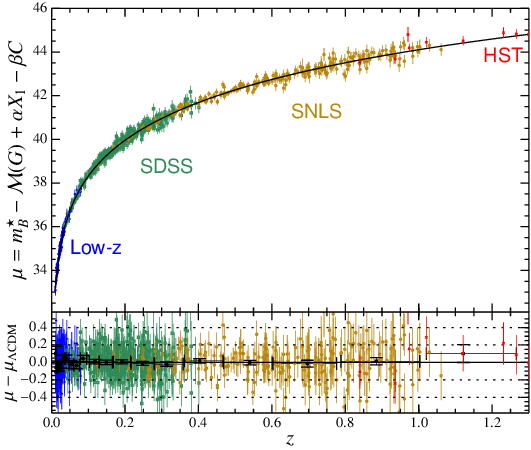
\includegraphics[width=\textwidth]{Figures/Chapter1/Betoule14Hubble.png}
  \caption{An example of a Hubble diagram reproduced from the Joint Light curve Analysis project \citep{Betoule2014}. $\sim$700 SN\,Ia form part of the sample which combines obects from the SNLS, SDSS, HST as well as low redshift SN observed by miscelenious instruments.}
  \label{fig:Betoule14Hubble}
\end{figure}

One of the largest problems with using SNe as cosmological probes is the difficulty of detecting these objects at redshifts higher than z$>$0.6 due to the majority of their optical flux being redshifted into IR bands where our ground-based telescopes are less sensitive \citep{Smith2018}. It is perhaps not surprising that the possibility of SLSNe, which do not suffer from the same issues, possibly acting as standardisable candles \citep{Inserra2014,Papadopoulus2015,Inserra2018a} has propelled the interest in the new class of luminous transients.

While still a subject to active debate, the most promising route towards their standardisation, presented in \citet{Inserra2018a}, suggests that absolute luminosity of SLSNe is inversely proportional to their decline time in a near inverse Phillips relation. Currently, these type of analysis are difficult to undertake due to the low number of complete and low redshift samples of objects, however, early indications do suggest a standardizability similar to those found in the early publication on the width-luminosity relationship of SN\,Ia \citep{Inserra2018a}.

\subsection{Redshift as a distance measure}
In SN research, in alignment with most branches of Astronomy, distance measurements are crucial for nearly all analysis. As SN are extremely distant and often associated with faint galaxies that are undetectable, redshift is often the only possible measure of their separation from us, the observers.

In the context of an expanding universe, distance can be defined in three ways; proper distance or the distance between the object and the observer at the point when the signal was received, comoving distance (D$_A$) which is the separation between the source and observer at the point the signal was emitted or luminosity distance (D$_L$), corresponding to the distance traveled by the light signal. The latter is the measure used in astronomy as it directly corresponds to the distance modulus, defining the relationship between the absolute (M) and the apparent (m) magnitudes of an object with distance:

\begin{equation}
  m = M + 5log(\frac{D_L}{10pc})
\end{equation}

Redshift and distance are not linearly proportional to each other and depend very strongly on the cosmological model used and its parameters. Throughout this thesis I use \eref{eq:LumDist} to compute all distances in conjucntion with the standard cosmology defined as: H$_0$ = 70$\mathrm{Km}\,\mathrm{s}^{-1}\,\mathrm{Mpc}^{-1}$, $\omega_M = 0.3$, $\omega_{\Lambda} = 0.3$

\begin{equation} \label{eq:LumDist}
  D_L = (1+z) \times \frac{c}{H_0} \int^{z}_{0} \frac{dz}{\sqrt{(1+z)^3 \omega_M + \omega_{\Lambda}}}
\end{equation}

\section{Thesis overview}
The overarching goal of this thesis is to demonstrate our ability to photometrically select SLSNe amongst the samples of transients detected by large astronomical surveys, focusing on the detection of the most distant objects of the class. This thesis is laid out as follows:

In \cref{Chapter2}, I introduce the surveys and other auxiliary data sources used in this thesis. I also present the sample of spectroscopically confirmed SLSN from Dark Energy Survey and introduce a sample of literature objects used as templates for their class. Following from this, \cref{Chapter3} describes a number of techniques and analytical frameworks, as well as packages designed to study and simulate artificial samples of both SLSNe and CCSNe. As part of this, I introduce the spin-down of the magnetar model, in the context of modelling the light curves of SLSNe, as well as a technique for enhancing the blackbody approximation of the SLSN SED to account for a number of absorption features commonly associated with this class.

\cref{Chapter4} builds upon the models and techniques developed in \cref{Chapter3} to produce a definition of SLSN in the context of the spin-down of a magnetar model. This is then applied to the archival SNLS data identifying one, previously unclassified SLSN. Together with the sample of additional two, spectroscopically confirmed object, they formed the base for a calculation of the rate of SLSN at z$\sim$1.

In \cref{Chapter5}, I discuss the possibility and the drawbacks of using a similar technique to detect SLSN in DES. Upon demonstrating that a novel Machine Learning approach is required, I discuss the development of artificial samples of SN light curves of all common classes as well as AGN and spurious survey noise, before applying it as a training sample for a Convolutional Neural Network powered photometric SN classifier. This model is then applied to the sample of real DES transients, first producing a pure sample of SNe before identifying a sample of potential SLSN candidates.

\cref{Chapter6} analyses the sample produced in \cref{Chapter5}. As it was shown that it suffers from contamination with SNIIP, the first step is to purify and select the strongest SLSN candidates. The observation properties of the sample are then briefly analysed before discussing its implications on the study of high redshift SLSN. Finally, \cref{Chapter7} summarises this thesis, highlights and concluding all the major finding as well as provides a forward look at what new surveys, such as LSST, will bring to the field of SLSNe.
